\chapter{Módulos del limitador} \label{append:programas}

En este anexo se presentan los módulos del limitador bajo un enfoque técnico. Para cada uno de los programas se adjunto su diagrama de clases (simplificado) y sus interfaces de entrada y salida de datos. Estos programas los discriminamos por re-utilizados y legacy, dependiendo de si forman parte del nuevo software o no.

\section{Módulos re-utilizados}

Estos programas han sido sometidos a una revisión de calidad mediante la cual se ha re-extructurado el código o se han re-implementado clases enteras, pero su diseño y su funcionamiento se han mantenido intactos.

\subsection{getConfig} \label{append:getConfig}
%\chapter{Recuperación de información: getConfig} \label{append:getConfig}

\begin{center}
    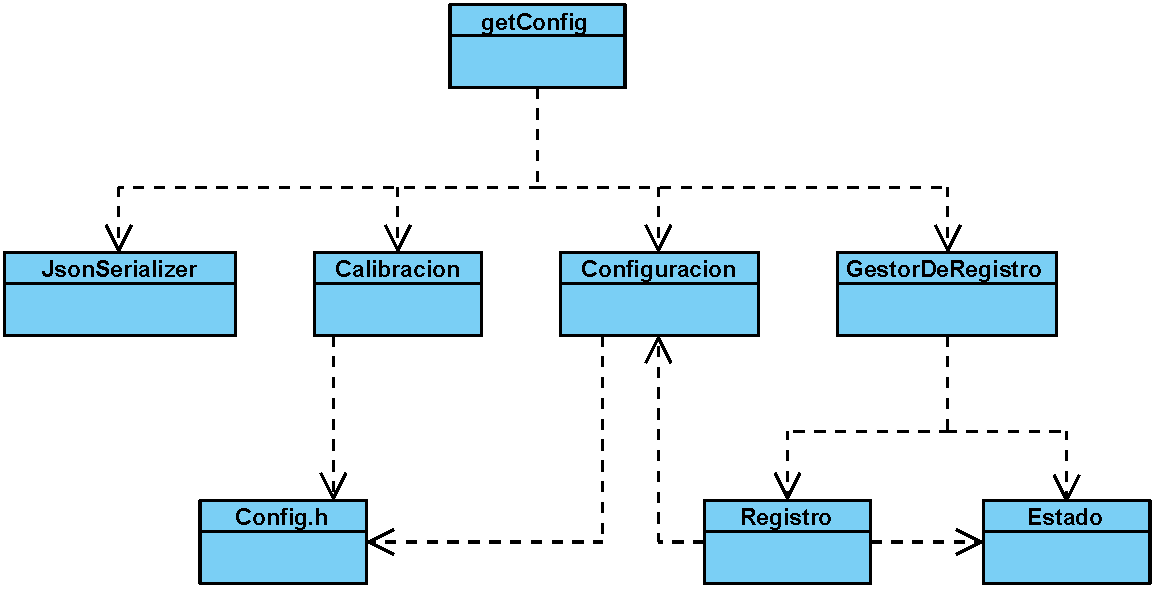
\includegraphics[width=0.9\textwidth]{figuras/lms11-getConfig.pdf}
    \captionof{figure}{Diagrama de clases del programa getConfig}
    \label{fig:getConfig}
\end{center}

El programa \verb|getConfig| devuelve la configuración del limitador en formato JSON. Para ello, accede a la información alojada en varios ficheros del sistema. Los ficheros a los que accede, así como el conjunto de datos que devuelve el programa pueden consultarse en los listados que se muestran a continuación en este anexo.

Ficheros:
\begin{multicols}{2}
	\begin{itemize}
	    \item \verb|/var/slr/configuracion|
	    \item \verb|/var/slr/registro.slr|
	    \item \verb|/var/slr/calibration[i]|
	    \begin{itemize}
	        \item 0: micrófono.
	        \item 1: línea izquierda.
	        \item 1: línea derecha.
	    \end{itemize}
	\end{itemize}
\end{multicols}

Datos:
\begin{multicols}{2}
	\begin{itemize}
	    \item Calibraciones.
	    \item Normativa.
	    \item Datos del local.
	    \item Tipo de equipo.
	    \item Propiedades del compresor.
	    \item Umbral de sesiones.
	    \item Aislamiento.
	    \item Versión del software.
	    \item Número de serie del equipo.
	    \item Fecha y hora del sistema.
	    \item Fecha y hora base del registro.
	\end{itemize}
\end{multicols}

%\begin{figure}[h]
%    \begin{minipage}[t]{.45\textwidth}
%        \begin{itemize}
%            \item Calibraciones.
%            \item Normativa.
%            \item Datos del local.
%            \item Tipo de equipo.
%            \item Propiedades del compresor.
%            \item Umbral de sesiones.
%        \end{itemize}
%    \end{minipage}
%    \hfill
%    \begin{minipage}[t]{.45\textwidth}
%        \begin{itemize}
%            \item Aislamiento.
%            \item Versión del software.
%            \item Número de serie del equipo.
%            \item Fecha y hora del sistema.
%            \item Fecha y hora base del registro.
%        \end{itemize}
%    \end{minipage}
%\end{figure}

% Fuerza la impresión de los floats pendientes hasta este punto.
\clearpage

\begin{lstlisting}[
    language=json,
    label={lst:lm7-getStatus},
    caption={Esquema JSON devuelto por getConfig en la versión LM7.}
]
{
  "definitions": {
    "data": {
      "type": "object",
      "properties": {
        "serialNumber": {
          "type": "integer"
        },
        "version": {
          "type": "number"
        },
        "time": {
          "type": "string"
        },
        "configTime": {
          "type": "string"
        },
        "place": {
          "type": "string"
        },
        "establishment": {
          "type": "string"
        },
        "address": {
          "type": "string"
        },
        "council": {
          "type": "string"
        },
        "responsible": {
          "type": "string"
        },
        "phonenumber": {
          "type": "string"
        },
        "vendor": {
          "type": "string"
        },
        "dayStartHour": {
          "type": "integer"
        },
        "dayEndHour": {
          "type": "integer"
        },
        "dayMaximumEmission": {
          "type": "number"
        },
        "nightMaximumEmission": {
          "type": "number"
        },
        "dayMaximumReception": {
          "type": "number"
        },
        "nightMaximumReception": {
          "type": "number"
        },
        "plainIsolation": {
          "type": "number"
        },
        "minumum": {
          "type": "number"
        },
        "maximum": {
          "type": "number"
        },
        "maximumattenuation": {
          "type": "integer"
        },
        "compressorRange": {
          "type": "number"
        },
        "compressorEfectivity": {
          "type": "integer"
        },
        "laeqtime": {
          "type": "integer"
        },
        "recoverTime": {
          "type": "integer"
        },
        "registryStartTime": {
          "type": "string"
        },
        "deviceType": {
          "type": "string"
        }
      }
    }
  }
}
\end{lstlisting}

\vspace{1em}

\begin{lstlisting}[
    language=json,
    label={lst:lm7-getStatus},
    caption={Esquema JSON devuelto por getConfig en las versiones LM9 y LM11.}
]
{
  "definitions": {
    "data": {
      "type": "object",
      "properties": {
        "serialNumber": {
          "type": "string"
        },
        "version": {
          "type": "string"
        },
        "time": {
          "type": "string"
        },
        "configtime": {
          "type": "string"
        },
        "activeSince": {
          "type": "string"
        },
        "registryBaseTime": {
          "type": "string"
        },
        "minimum": {
          "type": "number"
        },
        "maximum": {
          "type": "number"
        },
        "recoverTime": {
          "type": "integer"
        },
        "maximumAttenuation": {
          "type": "integer"
        },
        "maximumBandAttenuation": {
          "type": "number"
        },
        "minimalAttenuation": {
          "type": "number"
        },
        "thressholdCoefficient": {
          "type": "number"
        },
        "attenuationSteps": {
          "type": "integer"
        },
        "laeqTime": {
          "type": "integer"
        },
        "dayStartHour": {
          "type": "integer"
        },
        "dayEndHour": {
          "type": "integer"
        },
        "dayMaximumEmission": {
          "type": "number"
        },
        "nightMaximumEmission": {
          "type": "number"
        },
        "dayMaximumReception": {
          "type": "number"
        },
        "nightMaximumReception": {
          "type": "number"
        },
        "compressorRange": {
          "type": "number"
        },
        "compressorEfectivity": {
          "type": "integer"
        },
        "isolation": {
          "type": "array",
          "items": {
            "type": "number"
          }
        },
        "margins": {
          "type": "array",
          "items": {
            "type": "number"
          }
        },
        "controlType": {
          "type": "string"
        },
        "usePredictiveModel": {
          "type": "boolean"
        },
        "useReceptionControl": {
          "type": "boolean"
        },
        "audioBlocking": {
          "type": "boolean"
        },
        "useFrecuentialControl": {
          "type": "boolean"
        },
        "controlEachFrequency": {
          "type": "boolean"
        },
        "establishment": {
          "type": "string"
        },
        "address": {
          "type": "string"
        },
        "council": {
          "type": "string"
        },
        "responsible": {
          "type": "string"
        },
        "phonenumber": {
          "type": "string"
        },
        "vendor": {
          "type": "string"
        },
        "equipment": {
          "type": "string"
        },
        "activeDaysAfterConfiguration": {
          "type": "integer"
        },
        "daysOff": {
          "type": "array",
          "items": {
            "$ref": "#/definitions/DaysOff"
          }
        },
        "weekDayEmisionMaximum": {
          "type": "array",
          "items": {
            "type": "number"
          }
        },
        "weekNightEmisionMaximum": {
          "type": "array",
          "items": {
            "type": "number"
          }
        },
        "weekDayReceptionMaximum": {
          "type": "array",
          "items": {
            "type": "number"
          }
        },
        "weekNightReceptionMaximum": {
          "type": "array",
          "items": {
            "type": "number"
          }
        },
        "useExtendedNormative": {
          "type": "boolean"
        },
        "deviceType": {
          "type": "string"
        },
        "pinkNoiseLevel": {
          "type": "number"
        },
        "sessionStartThreshold": {
          "type": "number"
        },
        "sessionEndThreshold": {
          "type": "number"
        },
        "calibrations": {
          "type": "array",
          "items": {
            "$ref": "#/definitions/Calibration"
          }
        }
      }
    },
    "Calibration": {
      "type": "object",
      "properties": {
        "deviceNumber": {
          "type": "integer"
        },
        "dbRef": {
          "type": "number"
        },
        "referentia": {
          "type": "number"
        },
        "noiselevel": {
          "type": "number"
        },
        "hardwareLevel": {
          "type": "number"
        },
        "referenciaGlobal": {
          "type": "number"
        },
        "equalization": {
          "type": "array",
          "items": {
            "type": "number"
          }
        },
        "internalEqualization": {
          "type": "array",
          "items": {
            "type": "number"
          }
        }
      }
    },
    "DaysOff": {
      "type": "object",
      "properties": {
        "type": {
          "type": "integer"
        },
        "day": {
          "type": "integer"
        },
        "month": {
          "type": "integer"
        },
        "weekDayNumber": {
          "type": "integer"
        },
        "startHour": {
          "type": "integer"
        },
        "startMinutes": {
          "type": "integer"
        },
        "durationHours": {
          "type": "integer"
        },
        "durationMinutes": {
          "type": "integer"
        },
        "emissionMaximum": {
          "type": "number"
        },
        "receptionMaximum": {
          "type": "number"
        }
      }
    }
  }
}
\end{lstlisting}

%Esquemas generados a partir de muestras JSON del programa, mediante el uso de las herramientas \url{www.json-schema.org} y \url{www.jsonschemavalidator.net}.
\clearpage

\subsection{getStatus} \label{append:getStatus}
%\chapter{Recuperación de información: getStatus} \label{append:getStatus}

\begin{center}
    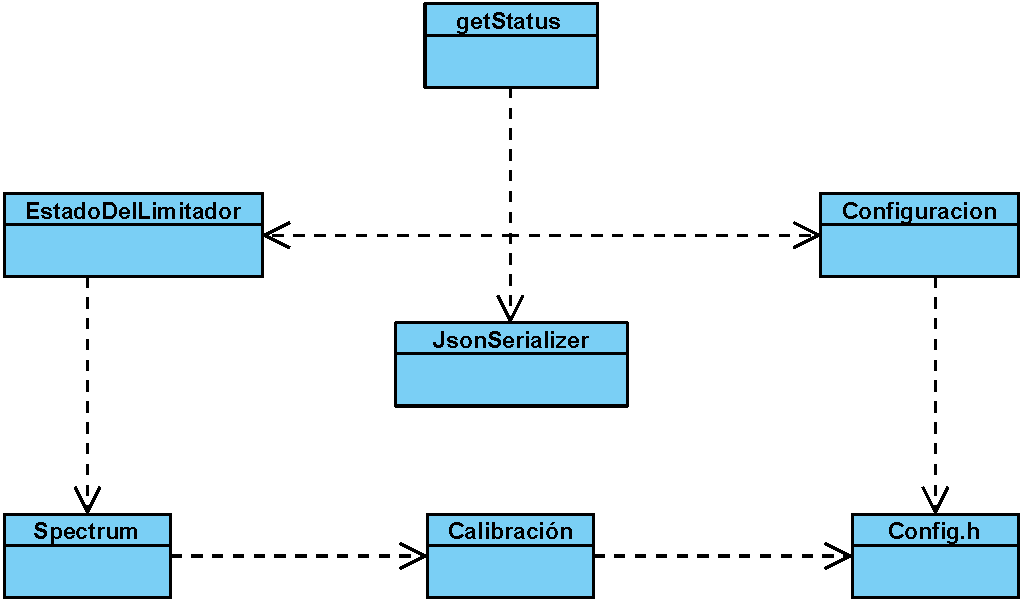
\includegraphics[width=0.9\textwidth]{figuras/lms11-getStatus.pdf}
    \captionof{figure}{Diagrama de clases del programa getStatus}
    \label{fig:getStatus}
\end{center}

El programa \verb|getStatus| devuelve información sobre el estado del limitador en el momento de la llamada. Para ello, lee el fichero \verb|/tmp/estado.slr| y devuelve su contenido en formato JSON. El fichero \verb|/tmp/estado.slr| es mantenido por el proceso de limitación en el caso del LM7, o por el proceso registrador en el caso del LM9 y el LM11.

En la figura \ref{fig:getStatus} se muestra el diagrama de clases simplificado del programa.

Los listados \ref{lst:lm7-getStatus} y \ref{lst:lm9-getStatus} muestran los esquemas JSON devueltos por este programa en cada una de las versiones. \\

\begin{lstlisting}[
    language=json,
    label={lst:lm7-getStatus},
    caption={Esquema JSON devuelto por getStatus en la versión LM7.}
]
{
  "definitions": {
    "data": {
      "type": "object",
      "properties": {
        "serialNumber": {
          "type": "string",
          "format": "integer"
        },
        "version": {
          "type": "string"
        },
        "time": {
          "type": "string"
        },
        "configTime": {
          "type": "string"
        },
        "place": {
          "type": "string"
        },
        "direction": {
          "type": "string"
        },
        "council": {
          "type": "string"
        },
        "responsible": {
          "type": "string"
        },
        "phoneNumber": {
          "type": "string"
        },
        "vendor": {
          "type": "string"
        },
        "deviceType": {
          "type": "string"
        },
        "leftline": {
          "type": "string"
        },
        "rightline": {
          "type": "string"
        },
        "microphone": {
          "type": "string"
        },
        "maximum": {
          "type": "string"
        },
        "microphoneConnected": {
          "type": "string"
        },
        "running": {
          "type": "string",
          "format": "integer"
        },
        "attenuation": {
          "type": "integer"
        },
        "micSpectrum": {
          "type": "array",
          "items": {
            "type": "number"
          }
        },
        "leftSpectrum": {
          "type": "array",
          "items": {
            "type": "number"
          }
        },
        "rightSpectrum": {
          "type": "array",
          "items": {
            "type": "number"
          }
        }
      }
    }
  }
}
\end{lstlisting}

\vspace{1em}

\begin{lstlisting}[
    language=json,
    label={lst:lm9-getStatus},
    caption={Esquema JSON devuelto por getStatus en las versiones LM9 y LM11.}
]
{
  "definitions": {
    "data": {
      "type": "object",
      "properties": {
        "time": {
          "type": "string",
          "format": "date-time"
        },
        "attenuation": {
          "type": "number"
        },
        "isActive": {
          "type": "boolean"
        },
        "running": {
          "type": "boolean"
        },
        "microphoneConnected": {
          "type": "boolean"
        },
        "maximum": {
          "type": "number"
        },
        "serialNumber": {
          "type": "string"
        },
        "version": {
          "type": "string"
        },
        "establishment": {
          "type": "string"
        },
        "address": {
          "type": "string"
        },
        "council": {
          "type": "string"
        },
        "responsible": {
          "type": "string"
        },
        "phonenumber": {
          "type": "string"
        },
        "configTime": {
          "type": "string"
        },
        "vendor": {
          "type": "string"
        },
        "deviceType": {
          "type": "string"
        },
        "noiseAttenuation": {
          "type": "number"
        },
        "noiseIsActive": {
          "type": "boolean"
        },
        "microphone": {
          "type": "number"
        },
        "leftline": {
          "type": "number"
        },
        "rightline": {
          "type": "number"
        },
        "mic": {
          "$ref": "#/definitions/spectrum"
        },
        "left": {
          "$ref": "#/definitions/spectrum"
        },
        "right": {
          "$ref": "#/definitions/spectrum"
        }
      }
    },
    "spectrum": {
      "type": "object",
      "properties": {
        "energy": {
          "type": "array",
          "items": {
            "type": "number"
          }
        },
        "dB": {
          "type": "array",
          "items": {
            "type": "number"
          }
        },
        "aWeighted": {
          "type": "array",
          "items": {
            "type": "number"
          }
        },
        "globaldB": {
          "type": "number"
        },
        "dBA": {
          "type": "number"
        }
      }
    }
  }
}
\end{lstlisting}

%Esquemas generados a partir de muestras JSON del programa, mediante el uso de las herramientas \url{www.json-schema.org} y \url{www.jsonschemavalidator.net}.
\clearpage

\subsection{getData} \label{append:getData}
%\chapter{Recuperación de información: getData} \label{append:getData}

\begin{center}
    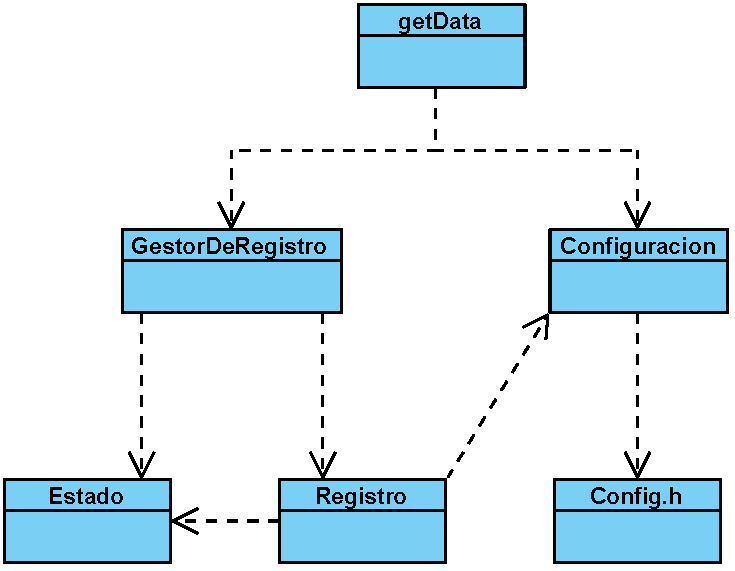
\includegraphics[width=0.9\textwidth]{figuras/lms11-getData.pdf}
    \captionof{figure}{Diagrama de clases del programa getData.}
    \label{fig:getData}
\end{center}

El programa \verb|getData| se encarga de recuperar los registros almacenados por el limitador pertenecientes a un intervalo de tiempo determinado, devolviéndolos en formato JSON. \verb|getData| recibe 4 parámetros y la sintáxis para invocarlo es la siguiente: \\

\begin{center}
    \verb|./getData $formato $fechaIni $fechaFin $intervalo|
\end{center}

donde:

\begin{itemize}
    \item Formato: \acrshort{XML} o \acrshort{JSON}
    \item Fecha de inicio: desde la fecha base del registro hasta la fecha actual.
    \item Fecha de fin: desde la fecha de inicio hasta la fecha actual.
    \item Intervalo de muestreo: intervalo de tiempo entre cada registro, en minutos.
\end{itemize}
La fechas van en el formato \verb|YYYY/MM/DD-hh:mm|, siguiendo el estándar \textbf{ISO 8601}.

Los listados \ref{lst:lm7-getData} y \ref{lst:lm9-getData} muestran los esquemas JSON devueltos por este programa en cada una de las versiones. \\
\begin{lstlisting}[
    language=json,
    label={lst:lm7-getData},
    caption={Esquema JSON devuelto por getData en las versión LM7.}
]
{
  "definitions": {
    "data": {
      "type": "object",
      "properties": {
        "registries": {
          "type": "array",
          "items": {
            "$ref": "#/definitions/Registry"
          }
        }
      }
    },
    "Registry": {
      "type": "object",
      "properties": {
        "time": {
          "type": "string"
        },
        "mic": {
          "type": "number"
        },
        "leftline": {
          "type": "number"
        },
        "rightline": {
          "type": "number"
        },
        "attenuation": {
          "type": "integer"
        },
        "maximum": {
          "type": "number"
        },
        "disconnectedMicrophone": {
          "type": "string",
          "format": "integer"
        }
      }
    }
  }
}
\end{lstlisting}

\vspace{1em}

\begin{lstlisting}[
    language=json,
    label={lst:lm9-getData},
    caption={Esquema JSON devuelto por getData en las versiones LM9 y LM11.}
]
{
  "definitions": {
    "data": {
      "type": "object",
      "properties": {
        "registries": {
          "type": "array",
          "items": {
            "$ref": "#/definitions/Registry"
          }
        }
      }
    },
    "Registry": {
      "type": "object",
      "properties": {
        "time": {
          "type": "string"
        },
        "mic": {
          "type": "number"
        },
        "leftline": {
          "type": "number"
        },
        "rightline": {
          "type": "number"
        },
        "attenuation": {
          "type": "integer"
        },
        "maximum": {
          "type": "number"
        },
        "disconnectedMicrophone": {
          "type": "string",
          "format": "integer"
        },
        "microphone": {
          "type": "array",
          "items": {
            "type": "number"
          }
        },
        "left": {
          "type": "array",
          "items": {
            "type": "number"
          }
        },
        "right": {
          "type": "array",
          "items": {
            "type": "number"
          }
        }
      }
    }
  }
}
\end{lstlisting}

%Esquemas generados a partir de muestras JSON del programa, mediante el uso de las herramientas \url{www.json-schema.org} y \url{www.jsonschemavalidator.net}.
\clearpage

\subsection{Configurador}

\clearpage

\section{Módulos legacy}

Estos programas no han sido seleccionados para formar parte del nuevo software, bien por su excesiva complejidad, funcionalidad duplicada o no requerida, o mezcla de ambas cosas.

\subsection{limInfo} \label{append:limInfo}
%\chapter{Recuperación de información: limInfo} \label{append:limInfo}

\begin{center}
    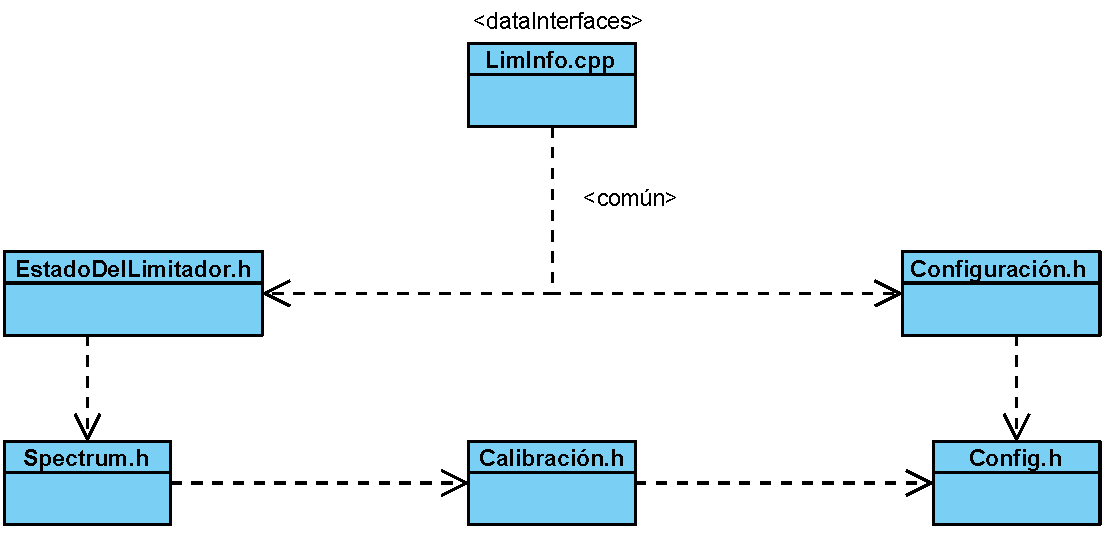
\includegraphics[width=0.9\textwidth]{figuras/lms9-limInfo.pdf}
    \captionof{figure}{Diagrama de dependencias del programa limInfo.}
    \label{fig:limInfo}
\end{center}

El programa recibe como parámetro una cadena de caracteres, en la que cada carácter corresponde a la consulta de una propiedad del limitador. En el listado de códigos de este anexo se muestra la información que exporta el programa \verb|limInfo| y el carácter necesario para su consulta.

En la figura \ref{fig:limInfo} se muestra el diagrama de dependencias del programa. Este diagrama representa la inclusión de otros ficheros de código fuente C++ en el fichero \verb|limInfo.cpp|. Estas inclusiones no siempre son clases, por lo que \textbf{no debe confundirse con un diagrama de clases}. En las relaciones se muestra entre ángulos el módulo al que pertenece (la carpeta en la que se encuentra dentro del proyecto).

Este programa se consideró redundante ya que se puede obtener la misma información mediante el \verb|getConfig|, por lo que no ha sido exportado ni utilizado por nuestro sistema.

Leyenda:
\begin{itemize}
    \item El símbolo igual (=) indica cuál es el valor por defecto de la propiedad a la que acompaña.
    \item La flecha hacia la derecha ($\rightarrow$) da comienzo a un comentario sobre la propiedad que la precede.
    \item La flecha en ambos sentidos ($\leftrightarrow$) indica que esa propiedad está duplicada.
\end{itemize}

Códigos:
\begin{itemize}
    \item A: configuración.atenuaciónMáxima = 90
    \item I: configuración.normativa.intervalo.horaInicio
    \item F: configuración.normativa.intervalo.horaFin
    \item D: configuración.normativa.máximoDiurno
    \item N: configuración.normativa.máximoNocturno
    \item \{: configuración.normativa.máximoRecepciónNocturno
    \item \}: configuración.normativa.máximoRecepciónDiurno
    \item T: configuración.tiempoBajoMáximo = 5 $\rightarrow$ cada cuánto reduce la atenuación si no hay subidas.
    \item P: configuración.pasos = 1 $\rightarrow$ pasos de atenuación por cada segundo que se sobrepasa el máximo.
    \item E: configuración.penalización
    \item S: configuración.partesDeCompresor
    \item G: configuración.rangoDePenalización = 120
    \item I: configuración.activo
    \item @: configuración.local
    \item Q: configuración.medidasPorCiclo = 2
    \item C: configuración.tipoDeControl $\rightarrow$ 0: Mic, 1: Líneas, 2: Mixto
    \item R: estado.recepción
    \item l: estado.presiónIzquierda
    \item L: estado.presiónDerecha
    \item n: configuración.númeroDeSerie
    \item v: configuración.versión
    \item f: enFuncionamiento
    \item p: estado.presión
    \item a: estado.atenuación
    \item d: estado.micrófonoConectado
    \item m: estado.media
    \item M: configuración.máximoEnEmisión(ahora)
    \item h: estado.hora
    \item s: configuración.servidorDeDatos
    \item r: configuración.horaDeReprogramado
    \item u: configuración.válido = true $\rightarrow$ Siempre es \verb|true|.
    \item 3: configuración.local $\leftrightarrow$ @
    \item 4: número de serie.
    \item 5: configuración.dirección
    \item 6: configuración.teléfono
    \item 7: configuración.persona
    \item 8: configuración.ayuntamiento
    \item 9: configuración.distribuidor
    \item .: configuración.predictivo
    \item ?: configuración.aislamiento
    \item X: número de serie + versión + presión + atenuación + media + máximo + hora + enFuncionamiento + horaReprogramado + atenuación máxima
\end{itemize}
\clearpage

\subsection{localService} \label{append:localservice}


\begin{center}
    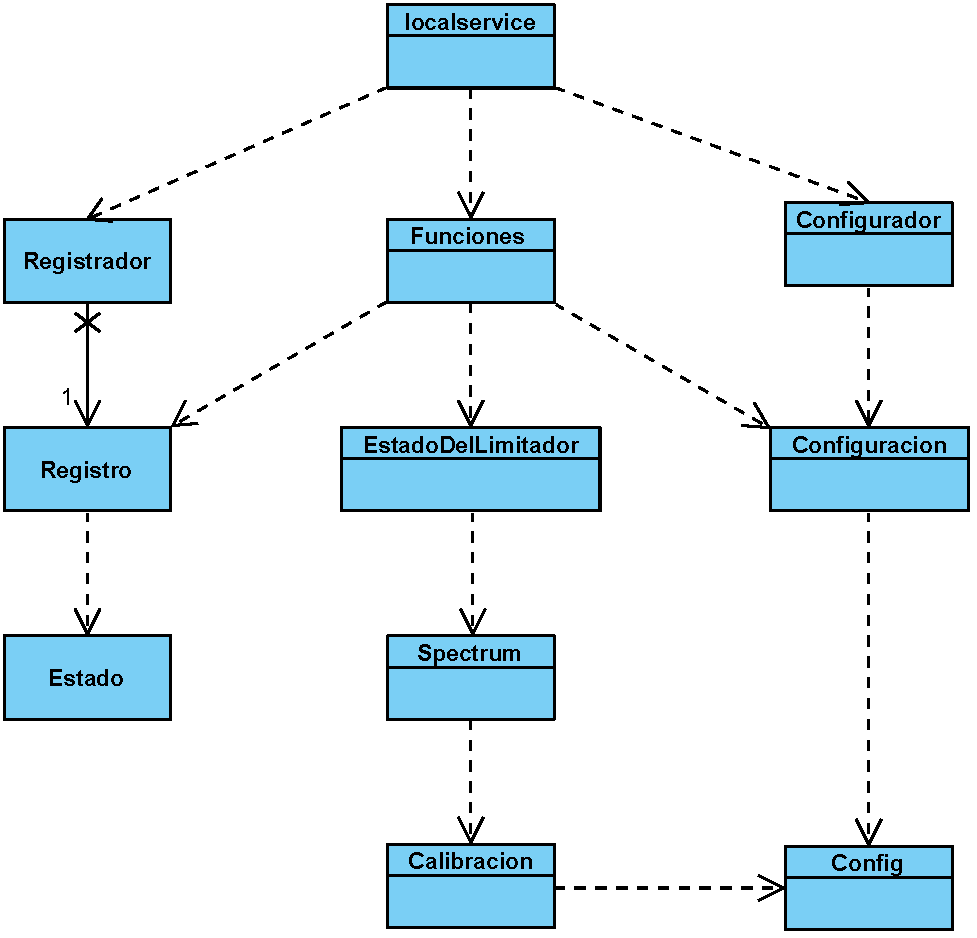
\includegraphics[width=0.9\textwidth]{figuras/lms9-localservice.pdf}
    \captionof{figure}{Diagrama de dependencias del programa localservice.}
    \label{fig:localservice}
\end{center}

Al igual que \verb|utilslr| recibe una serie de comandos como parámetro para modificar y consultar los datos del limitador. Los datos se devuelven \textbf{sin formato} útil (no JSON). El programa resulta excesivamente complejo, ya que contiene más del 1000 líneas de código, y ofrece funcionalidades que ya realizan otros de los programas auxiliares. Este programa pretende funcionar como un intérprete de comandos o una consola remota. Puede abrir y mantener un socket HTTP si se compila con las banderas requeridas.

Aunque el programa se llama \verb|localservice|, la clase principal se llama \verb|ServidorSerie|.

A continuación se listan los comandos que puede recibir este programa. Aquellos resaltados en negrita representan funcionalidad útil que ha sido exportada al LM11. Es fácil observar que mucha de las funcionalidades que ofrece este programa también la ofrecen otros programas auxiliares mucho menos complejos que este, y no solo eso, sino que mismamente dentro programa hay funcionalidad duplicada.

Comandos vía argumentos:
\begin{itemize}
	\item \textbf{calibralineas}: calibra el micrófono y las líneas.
	\item \textbf{miceq}: devuelve la ecualización del micrófono.
	\item \textbf{lefteq}: devuelve la ecualización de la línea izquierda.
	\item \textbf{righteq}: devuelve la ecualización de la línea derecha.
	\item \textbf{mic} \$float: re-calibra el micrófono con el valor recibido.
	\item \textbf{lefteq} \$float[8]: actualiza la ecualización de la línea izquierda con los valores recibidos.
		\subitem Los valores se dan separados por comas.
	\item \textbf{righteq} \$float[8]: actualiza la ecualización de la línea derecha con los valores recibidos.
		\subitem Los valores se dan separados por comas.
\end{itemize}

Comandos vía intérprete:
\begin{itemize}
	\item datos: permite modificar los datos del local.
	\item update: descarga y aplica la actualización dada una URL.
	\item configuración: muestra la configuración.
	\item configura: permite modificar parte de la configuración.
	\item actva: activa o desactiva el sistema.
	\item concha: abre conexión a telnet en el puerto 1036. Promociona la conexión.
	\item concharemota: abre conexión al terminal remoto en sheel.boanergesnetwork.com con la utilidad \verb|nc|.
	\item identifica: login.
	\item \textbf{calibra}: calibra un sensor manualmente.
	\item prepara:
		\begin{itemize}
			\item Muestra la configuración.
			\item Permite borrar la configuración.
			\item Permite cambiar datos del local.
			\item Permite inicializar el registro.
			\item Permite cambiar parte de la configuración.
		\end{itemize}
	\item operativo:
		\begin{itemize}
			\item Muestra la configuración.
			\item Permite cambiar algunos datos de la configuración.
		\end{itemize}
	\item \textbf{test}: calibra las líneas.
\end{itemize}
\clearpage

\subsection{utilslr} \label{append:utilslr}
%\chapter{Recuperación de información: limInfo} \label{append:limInfo}

\begin{center}
    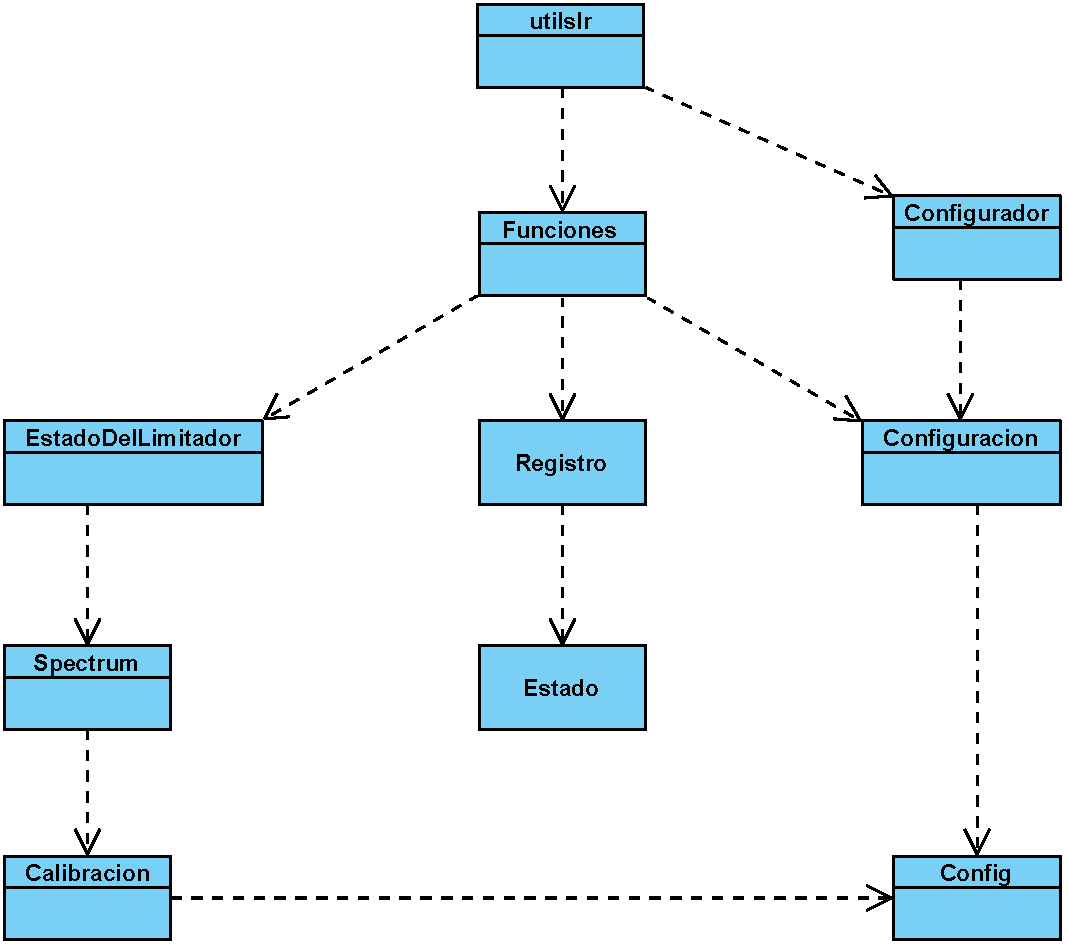
\includegraphics[width=0.9\textwidth]{figuras/lms9-utilslr.pdf}
    \captionof{figure}{Diagrama de dependencias del programa utilslr.}
    \label{fig:utilslr}
\end{center}

El programa \verb|utilslr| recibe serie de comandos como parámetro, principalmente para modificar la configuración del equipo (con \verb|utilslr configura|), pero también para consultar información e incluso generar informes en varios formatos (aunque tras probarlos la mayoría no funcionan).

El programa \verb|utilslr| se usa de forma intensiva en la versión LM7, por parte de la aplicación web. Generalmente se usa para aplicar la configuración y comprobar las contraseñas de usuario.

A continuación se listan los comandos que puede recibir este programa. Aquellos resaltados en negrita representan funcionalidad útil que ha sido exportada al LM11.
\begin{itemize}
	\item clave \$p: comprueba si la contraseña p es correcta.
	\item activaweb \$código \$nSerie \$nDistribuidor: activa la aplicación web.
	\item configuración: devuelve la configuración del equipo, igual que \verb|getConfig|.
	\item \textbf{configura} \$fichero: aplica la configuración definida en el fichero indicado (siempre es \verb|/tmp/conf.tmp|).
	\item \textbraceleft preauth, verifycu\textbraceright: relacionados con verificación de usuarios nuevos. Carecen totalmente de interés para nuestro proyecto.
	\item \textbraceleft sql, xml, yml, json, sqlite\textbraceright  \$fechaIni \$fechaFin \$intervalo: genera volcados en el formato indicado. Solo funcionan sql, xml y json.
	\item \textbraceleft listado, gráfico, actividad\textbraceright: sin usos conocidos.
\end{itemize}
\clearpage
